%!TEX root = ./thesis-main.tex
\chapter{Introduzione}\label{chap:introduction}
Nell'era digitale, il software pervade ogni aspetto della vita quotidiana. L'elemento che ha un impatto maggiore sull'esperienza di utilizzo è quasi sempre l'interfaccia utente. Riveste un ruolo chiave nella \textit{user experience},  influenzando in modo preponderante il giudizio complessivo sul prodotto finale. In un certo senso, è un aspetto che rende univoco qualsiasi software, determinando la sua efficacia e fruibilità. Rappresenta il punto d'incontro tra l'utente e le funzionalità del sistema stesso. Una \ac{UI} fluida e accessibile permette all'utente di esplorare tutte le funzionalità del software e di sfruttarne al meglio il potenziale. Essa non è solo un insieme di elementi estetici, ma un vero e proprio linguaggio visivo che comunica con l'utente e lo guida all'utilizzo.
\newline 
Per la conservazione di una esperienza utente soddisfacente, è fondamentale stare al passo delle tecnologie moderne. In un mondo in costante evoluzione, gli utenti si aspettano interfacce grafiche piacevoli e intuitive.
Da questa situazione emerge l'esigenza della creazione di una interfaccia web per il simulatore \textit{Alchemist}, in grado di affidarsi alla nuova infrastruttura \ac{API}, sviluppata per l'accesso e controllo dei dati delle simulazioni. L'interfaccia grafica esaminata all'interno di questo elaborato è destinata a procurare un punto di partenza per descrivere il meta-modello di un sistema complesso come quello di Alchemist, mediante l'utilizzo di uno stile moderno e facile da usare.
\section{Contesto}
Il progresso tecnologico degli ultimi vent'anni converge sempre più alla totale integrazione di dispositivi connessi a Internet nella vita quotidiana. La società odierna dipende sempre di più dalla tecnologia per soddisfare le proprie esigenze, spesso ricorrendo all'utilizzo di apparati e servizi tra loro eterogenei in hardware, ma soprattutto in software. Smartphone, \textit{wearables}, dispositivi embedded, TV, elettrodomestici, e una vasta gamma di altre tecnologie contribuiscono a creare un ecosistema digitale interconnesso. In questo contesto nasce il concetto di \textit{Pervasive Computing}, un modello informatico proposto negli anni '80, quando il ricercatore Mark Weiser introdusse il concetto di ``computing ubiquo" (da qui anche la denominazione \textit{Ubiquitous Computing})~\cite{Weiser2002}.
L'obiettivo principale di questo paradigma è quindi quello di rendere la tecnologia meno intrusiva e più adattabile al contesto dell'utente.   Per raggiungere questo obiettivo, è necessario un coordinamento efficace dei dispositivi, che deve garantire un'integrazione armoniosa e una comunicazione fluida tra di essi per fornire un'esperienza priva di discontinuità. Un sistema di questo tipo deve presentare caratteristiche di adattabilità e auto-organizzazione.
L'ingegneria di questi sistemi si concentra sulla coordinazione di agenti mobili e interconnessi che collaborano attraverso lo scambio di informazioni.
\subsection{Simulazione}

Il ricorso a strumenti simulativi per studiare sistemi composti da entità in grado di auto-coordinarsi e scambiare informazioni con l'ambiente circostante risulta essere essenziale per validare modelli che rappresentano scenari diversi. Una simulazione consente di eseguire una serie di test in un ambiente isolato per garantire che i modelli producano risultati attendibili. Inoltre, è possibile valutare l'impatto delle prestazioni del sistema in situazioni con un'alta densità di agenti, nonché variazioni nella topologia di interconnessione o cambiamenti nei pattern di interazione. Una simulazione precede l'implementazione reale del sistema in esame, esponendo punti di forza e punti deboli in anticipo, riducendo così il rischio di errori potenzialmente costosi in risorse, tempo e denaro.
In questo ambito, Alchemist unisce la caratteristiche di una simulazione di tipo \textit{\ac{DES}} a un modello di tipo \textit{\ac{ABM}}~\cite{PMV2011}. Nel primo caso si tratta di un metodo per modellare e analizzare il comportamento di un sistema nel tempo. In questo tipo di simulazione, il tempo è suddiviso in unità discrete definite come \textit{step} e lo stato del sistema cambia solo in determinati istanti, in corrispondenza di eventi significativi.
Il secondo invece è un tipo di modello computazionale in cui i singoli agenti seguono regole e interagiscono tra loro e con l'ambiente circostante. Questi agenti possono rappresentare una vasta gamma di entità, consentendo alla simulazione di descrivere e analizzare fenomeni come il comportamento sociale, la dinamica del mercato o la diffusione di malattie. 

Questa combinazione permette di esplorare uno spettro esteso di scenari e di studiare fenomeni complessi in un ambiente controllato, fornendo risposte a domande di tipo \textit{``what-if"} e aiutando a comprendere gli effetti potenziali di varie situazioni ipotetiche.
\subsection{Alchemist}
Alchemist~\cite{Pianini_2013} è un framework di simulazione open-source progettato e sviluppato dall'Università di Bologna per supportare lo studio e l'analisi di sistemi pervasivi.  Il suo scopo principale è quello di fornire agli sviluppatori uno strumento avanzato per dettagliare e simulare interazioni complesse tra individui autonomi in ambienti dinamici e distribuiti. Gli agenti autonomi fanno parte di un ecosistema che evolve nel tempo in modo autogestito attraverso leggi di base (chiamate \textit{eco-laws}) che definiscono meccanismi di coordinamento, comunicazione e interazione. 
L'approccio intrapreso da Alchemist per le interazioni tra i nodi (agenti) si ispira a reazioni chimiche, la cui natura aleatoria deriva dall'implementazione di un \textit{\ac{SSA}} su misura~\cite{PMV2011}. Ne consegue  un comportamento indipendente da parte degli agenti all'interno del sistema, che rispecchiano le peculiarità mutevoli e intricate dei contesti pervasivi.
L'architettura del simulatore consente di modellare gli \textit{autonomous-agents} come entità che spaziano in diversi campi, tra cui il \textit{pervasive}, l'\textit{aggregate} e il \textit{nature-inspired computing}.

\subsubsection{Il meta-modello}
Con meta-modello ci si riferisce alla struttura concettuale che definisce le entità e le loro relazioni all'interno dell'ambiente di simulazione. Serve per delineare gli elementi fondamentali e le loro interazioni, fornendo una base per la costruzione ed esecuzione di simulazioni. In generale, è utile per definire e comprendere i componenti e le dinamiche del mondo simulato in Alchemist. Gli elementi principali sono i seguenti:

\begin{itemize}
	\item \textbf{Molecule}:  Denominazione di un determinato dato.
	\item \textbf{Concentration}:  Valore associato a una particolare \textbf{molecule}. 
	\item \textbf{Node}: Contenitore di molecole e reazioni, situato all'interno dell'ambiente di simulazione.
	\item \textbf{Environment}: Rappresenta lo spazio di simulazione. È un contenitore di nodi e può fornire informazioni su:
	\begin{enumerate}
		\item La posizione dei nodi nell'ambiente.
		\item La distanza tra due nodi.
		\item Il supporto allo spostamento dei nodi.
	\end{enumerate}
	\item \textbf{Linking rule}: Funzione dello stato corrente dell'\textbf{environment}, che associa a ciascun nodo un vicinato.
	\item \textbf{Neighborhood}: Entità definita da un nodo centrale e un insieme di nodi vicini a esso.
	\item \textbf{Reaction}\label{item:reactions}: Qualsiasi evento che può cambiare lo stato dell'ambiente. Ogni nodo ha un insieme di \textbf{reaction}, che può anche essere vuoto. Ogni reaction è definita da una lista di condizioni, una o più azioni e una distribuzione temporale. La frequenza con cui la \textbf{reaction} accade dipende da:
		\begin{enumerate}
		\item Un parametro di frequenza statico.
		\item Il valore di ogni \textbf{condition}.
		\item Una ``equazione di frequenza'' che combina il parametro di frequenza statico con il valore delle \textbf{condition}, fornendo come risultato una valore di ``frequenza istantanea''.
		\item Una valore di distribuzione temporale.
	\end{enumerate}
	\item \textbf{Condition}: Una funzione che prende in input lo stato corrente dell'ambiente e restituisce un valore booleano e un numero. Se la \textbf{condition} non è soddisfatta (ovvero il suo output ritorna falso), la \textbf{reaction} a cui è associata non può essere eseguita. La distribuzione temporale e il numero in output hanno la possibilità di influenzare o meno la velocità delle \textbf{reaction}.
	\item \textbf{Action}: Modella un cambiamento nell'ambiente.
\end{itemize}

La \cref{fig:alchemist-model} illustra il modello in esame\footnote{\url{https://alchemistsimulator.github.io/explanation/metamodel}}.

\begin{figure}
	\centering
	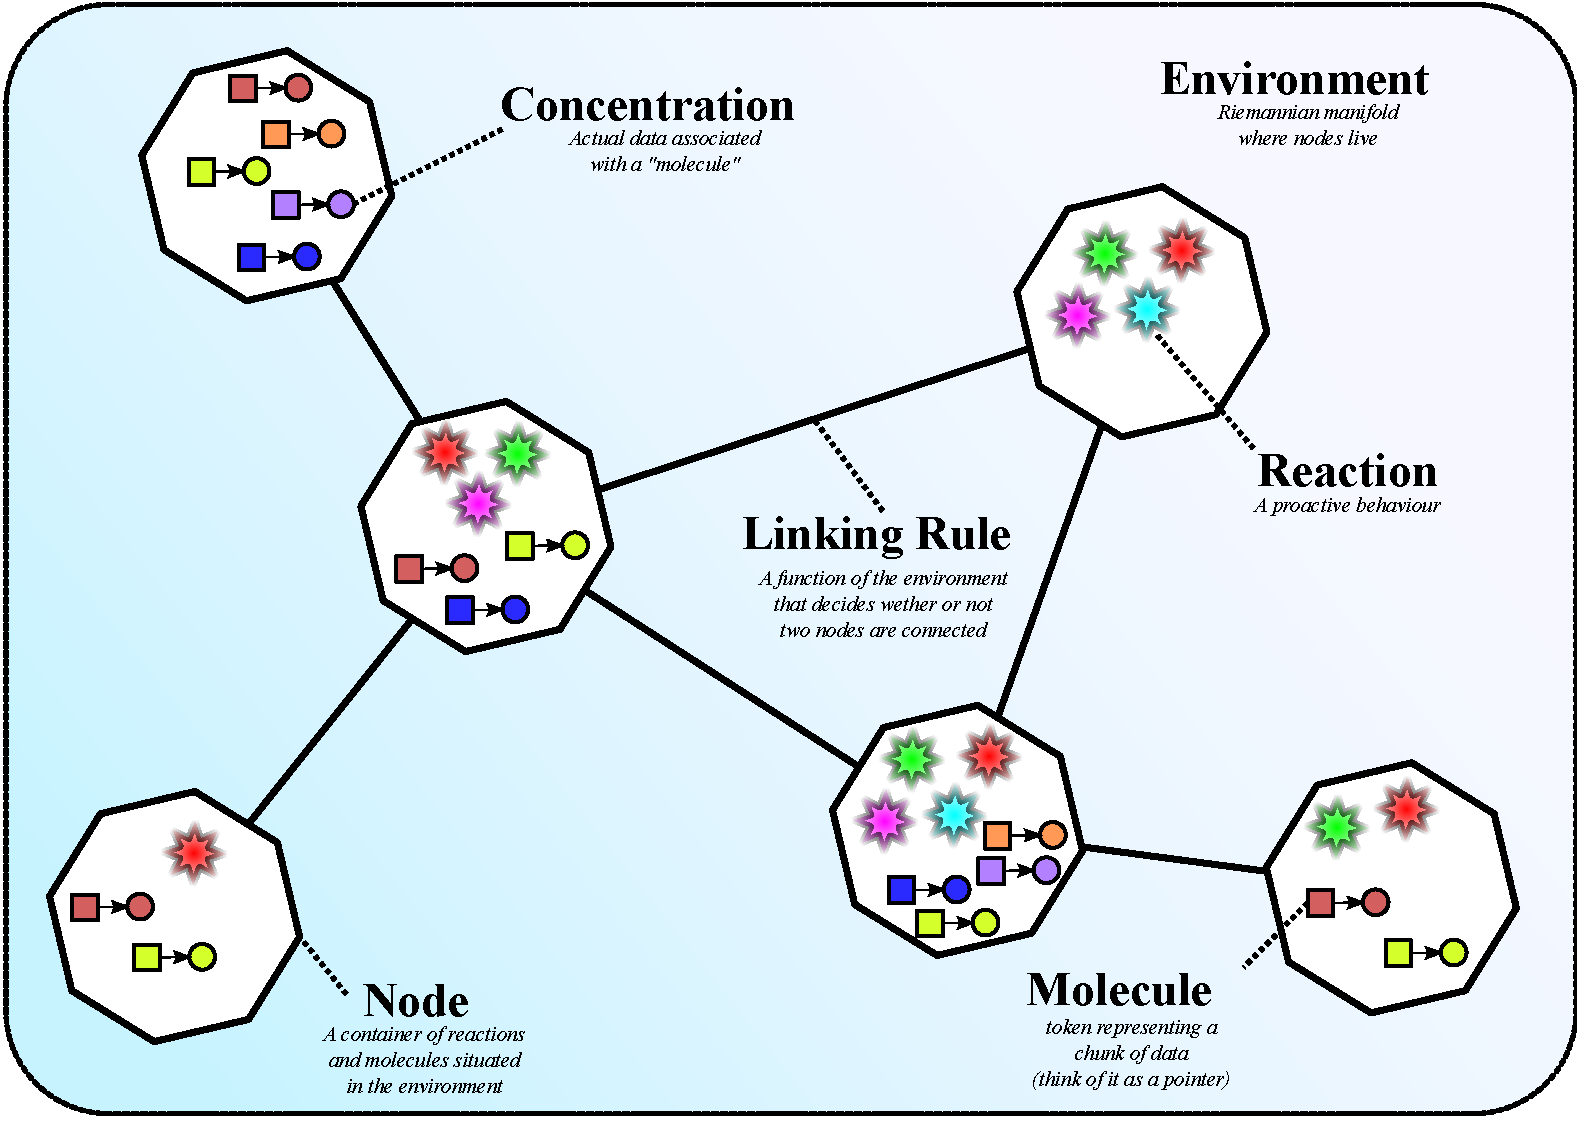
\includegraphics[width=.85\linewidth]{imgs/alchemist_meta_model.pdf}
	\caption{Rappresentazione del meta-modello di Alchemist}
	\label{fig:alchemist-model}
\end{figure}

\subsubsection{Incarnation}
Inizialmente Alchemist è stato concepito solamente come un motore di simulazione stocastico orientato alle reazioni chimiche, dando mobilità ai nodi e mantenendo alte prestazioni. 
La duttilità di questo simulatore risiede nella concezione generale di \textbf{molecule} e \textbf{concentration}. In Alchemist quest'ultimi sono definiti, rispettivamente, come un generico codice identificativo e un dato di un certo tipo. Una \textit{incarnation} definisce pertanto il tipo delle \textbf{concentration}, il set delle \textbf{condition} specifiche, le \textbf{action}, l'\textbf{environment} e le \textbf{reaction} che possono operare su tali tipi.
In altre parole, una incarnation è un'istanza concreta del meta-modello di Alchemist ed è per questo motivo che è possibile modellare scenari completamente diversi tra loro.
Al momento, le incarnation possibili sono le seguenti:
\begin{enumerate}
	\item \textbf{Protelis incarnation}~\cite{Pianini2015}:  progettato per semplificare la creazione di una rete composta da dispositivi potenzialmente mobili e diversi tra loro. Aderisce al paradigma di \textit{aggregate computing}, che applica la filosofia \textit{divide et impera} mediante l'utilizzo di una rete di sensori e computer distribuiti.
	\item \textbf{SAPERE incarnation}~\cite{Zambonelli2015}: progettato per la simulazione di sistemi compositi di servizi pervasivi.
	\item \textbf{Biochemistry incarnation}\footnote{\url{https://alchemistsimulator.github.io/explanation/biochemistry}}: consente di modellare reazioni chimiche o fenomeni biochimici all'interno dell'\textbf{environment}.
	\item \textbf{Scafi incarnation}~\cite{Casadei2022}:  progettato anch'esso per la simulazione di sistemi compositi di servizi pervasivi.
\end{enumerate}

\subsubsection{Scenari di utilizzo di Alchemist}
La verifica empirica delle funzionalità del simulatore in un contesto operativo è un passaggio ineluttabile per attestarne le capacità di esecuzione. Per acquisire una maggiore comprensione delle potenzialità e applicazioni di Alchemist, sono riportati alcuni casi d'uso che illustrano le diverse funzionalità del simulatore.

\begin{itemize}
	\item \textbf{2020: simulazione di \textit{crowd control} mediante dispositivi mobili a Torino}~\cite{Audrito2021}.
	Il caso di studio riguarda la sorveglianza della densità della folla nel Parco del Valentino a Torino tramite dispositivi indossabili e server \textit{''edge''} distribuiti nel parco. L'obiettivo del sistema è stato prevenire situazioni di sovraffollamento, stimando densità locale e baricentro della folla per notificare agli operatori sul campo aree potenzialmente pericolose. Sono stati impiegati nove server \textit{edge} posizionati strategicamente e il sistema è stato sottoposto a diverse condizioni realistiche, tra cui perdita di pacchetti e variazioni nella frequenza di funzionamento dei dispositivi.
	\item \textbf{2022: rilevamento e attuazione distribuita dei dati di pluviometri a Toronto}~\cite{Aguzzi_2022}.
	La simulazione si è concentrata sulla previsione della pioggia a Toronto utilizzando dati pubblici e una rete di sensori. Sono stati utilizzati 50 campioni di pioggia reali e 300 sensori simulati, interpolando i dati dei dispositivi circostanti. Gli algoritmi hanno valutato il rischio in base all'intensità della pioggia e all'altitudine locale, generando allerte in tempo reale. Le prestazioni sono state valutate attraverso il numero di allerte e le stazioni raggiunte.
 	\item \textbf{2022:  simulazione dell'affluenza alle attrazioni all'interno del parco divertimenti Mirabilandia}\footnote{\url{https://github.com/ICPS-MicroCity/amusement-park-simulation}}.
	L'obiettivo di questa simulazione è stato determinare se un sistema di raccomandazione possa influenzare positivamente il flusso dei visitatori in un parco divertimenti, confrontandolo con un sistema di re-indirizzamento casuale. I risultati mostrano che il sistema di raccomandazione adattivo può ridurre i tempi di attesa solo con un numero limitato di visitatori, mentre con un numero elevato i tempi di attesa aumentano significativamente rispetto alla politica di tipo random.
	\item \textbf{2022: simulazione degli avvenimenti di Piazza San Carlo del 2017}\footnote{\url{https://github.com/kelvin-olaiya/SanCarloSquareStampede}}.
	Lo studio si propone di capire le dinamiche che emergono durante un'evacuazione di emergenza in luoghi affollati, analizzando il disastro di Piazza San Carlo a Torino nel 2017. Simulando il comportamento delle persone e introducendo elementi di interazione fisica, la ricerca ha osservato come la paura si propaga nella folla (contagio sociale), creando un'onda di ``spinte'' simile a quella osservata durante l'evento reale. L'obiettivo è stato unire le conoscenze sulla psicologia umana nelle situazioni di panico con le interazioni fisiche per migliorare la gestione di eventi disastrosi in ambienti affollati.
\end{itemize}

\section{Motivazioni}
Nella scena del frontend, le tecnologie più all'avanguardia e in costante aggiornamento sono legate al web, dove le innovazioni si susseguono rapidamente per migliorare l'esperienza utente e l'efficienza di sviluppo. Anche le più grandi compagnie mondiali tengono costantemente aggiornato il design delle \ac{UI} dei loro prodotti, mantenendo vivo il loro fascino e adattandosi alle aspettative degli utenti. Alchemist dispone già di moduli in grado di rappresentare graficamente l'ambiente di simulazione. Sebbene le interfacce desktop offrono i loro vantaggi rispetto a quelle web, quest'ultime migliorano aspetti legati alla portabilità e interattività, permettendo di descrivere comportamenti più complicati,  presentare all'utente le informazioni sulla simulazione in modo creativo grazie all'utilizzo di librerie e framework moderni. Non solo: è possibile conferire alla \ac{UI} un comportamento responsivo, l'integrazione con altri servizi web o \ac{API} diventa più agevole, e viene richiesta la scrittura di un unico codice interpretabile da qualsiasi browser. L'esistenza di una piattaforma di \ac{API} capace di controllare e gestire la simulazione da un alto livello di astrazione getta le fondamenta per la necessità di creare un'interfaccia che sappia sfruttare appieno il potenziale offerto da tali funzionalità. 
\section{Obiettivi}
Il lavoro di questo progetto mira alla creazione di una interfaccia web che sfrutti le \ac{API} per il controllo e l'accesso ai dati della simulazione, consentendo all'utente di interagire con il sistema nel modo più intuitivo ed efficiente possibile. Il layout grafico deve allinearsi, preferibilmente, con le linee guida di design moderne, senza introdurre meccanismi fuorvianti o interazioni complicate e verbose. Questo contribuisce a interagire con il modello  di Alchemist nel modo più chiaro possibile, permettendo all'utente di comprendere e analizzare pienamente le dinamiche della simulazione.
In vista di un costante iter di miglioramenti e adattamenti futuri, la struttura dell'interfaccia deve agevolare la realizzazione di modifiche e l'aggiunta di nuove funzionalità, offrendo un ampio grado di espandibilità.
La \cref{fig:use-cases} raffigura il diagramma UML dei casi d'uso del modulo UI che andrà a integrarsi con le \ac{API} esistenti per presentare all'utente dati e informazioni concernenti la simulazione in corso. L'utente può controllare la simulazione avviandola o mettendola in pausa. Questi scenari estendono direttamente le funzionalità di controllo dell'infrastruttura di appoggio. Inoltre l'utente può ispezionare i nodi per visualizzarne il contenuto, oltre che ad assistere al progredire della simulazione stessa tramite la rappresentazione dei nodi in uno spazio bidimensionale. La concretizzazione di queste caratteristiche, invece, è possibile grazie al recupero in tempo reale delle informazioni necessarie a raffigurare lo scenario configurato.
\begin{figure}[htb]
	\centering
	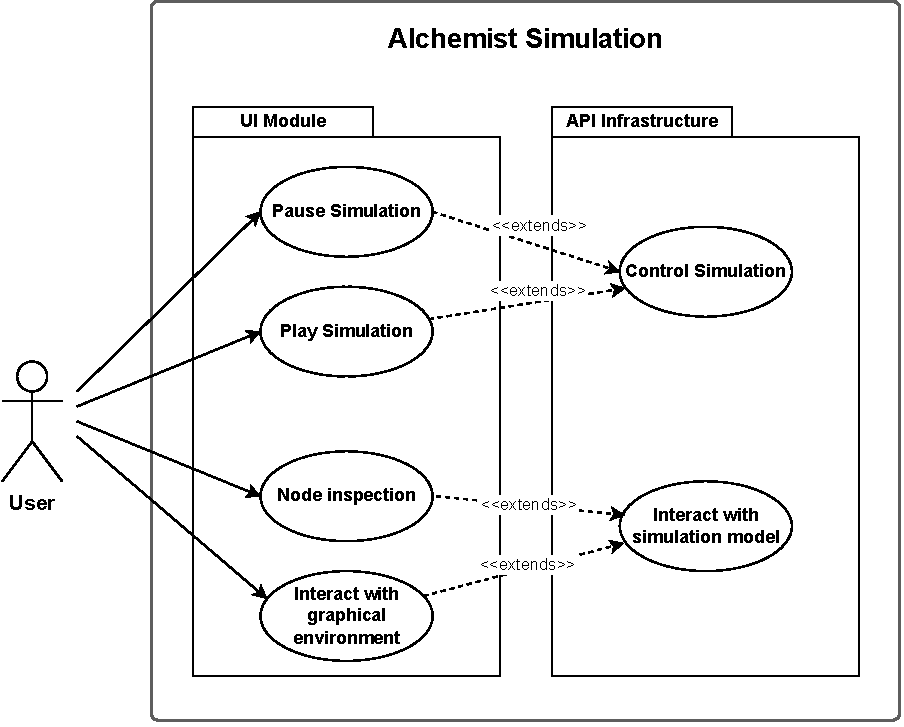
\includegraphics[width=.8\linewidth]{imgs/Use_cases.pdf}
	\caption{Diagramma UML dei casi d'uso del modulo UI per Alchemist}
	\label{fig:use-cases}
\end{figure}

